\documentclass[10pt,twocolumn]{article}

% ------------------ PAQUETES ------------------
\usepackage[spanish]{babel}
\usepackage[utf8]{inputenc}
\usepackage[T1]{fontenc}
\usepackage{geometry}
\usepackage{graphicx}
\usepackage{amsmath, amssymb}
\usepackage{siunitx}
\usepackage{authblk}
\usepackage{abstract}
\usepackage{caption}
\usepackage{titlesec}
\usepackage{multicol}
\usepackage{hyperref}
\usepackage{currfile}
\usepackage{float}

\geometry{margin=1.8cm}

% ------------------ FORMATO DE SECCIONES ------------------
\titleformat{\section}{\large\bfseries}{\thesection}{1em}{}
\titleformat{\subsection}{\normalsize\bfseries}{\thesubsection}{1em}{}

% ------------------ TÍTULO ------------------
\title{\textbf{Aproximación a las estrellas variables}\\Trabajo con métodos de machine learning para análisis de periodicidad\\Primer trabajo práctico de la serie}


% ------------------ AUTORES ------------------
\author[1]{Bruno Abello Laurent}

\affil[1]{Universidad de Los Andes, Departamento de Física, Colombia}

% Correos (puedes modificar)
\renewcommand\Authands{, }
\date{}

\begin{document}

\twocolumn[
\maketitle
\begin{center}
\small
\textit{Correo institucional:} \href{mailto:{b.abello@uniandes.edu.co}}{b.abello@uniandes.edu.co} \\
\textit{Repositorio de GitHub: } \href{https://github.com/Brunelleschk1/Personal-projects/tree/main/Proyectos\%20de\%20Astronom\%C3\%ADa/Laboratorio\%207}{Repositorio del laboratorio}
\end{center}

\begin{abstract}
\noindent
El presente informe es el segundo del autor con respecto a las estrellas variables, pero el primero en términos de conocimiento
práctico sobre el tema. Este documento se centra en el análisis del periodo mediante los métodos de Lomb Scargle y de mínima 
entropía de estrellas catalogadas en OGLE y en VVV. El objetivo fue realizar un análisis comparativo de los métodos, no un análisis 
de las estrellas como tal, puesto que el método que se siguió dió como resultados estrellas, en su mayoría, muy limpias en cuanto
al análisis de su periodo a primer orden. Análisis a órdenes más avanzados se realizarán en documentos posteriores
\end{abstract}

\noindent\textbf{Palabras clave:}
\vspace{0.5cm}
]

% ------------------ CONTENIDO ------------------

\section{Introducción}

Como se habló en el documento anterior, el mundo de las estrellas variables es sumamente extenso. El presente infore se centra en
estrellas variables de periodos cortos: no sabemos qué tipo de estrellas son exactamente, pero daremos respuestas parciales. 

\subsection{Objetivos}

Los objetivos que tenemos, en términos simples, son los siguientes:
\begin{itemize}
    \item Implementar una lectura sistemática de los datos de OGLE y VVV
    \item Analizar estrellas con Lomb Scargle y encontrar su periodo
    \item Analizar estrellas con Mínima Entropía y comparar esos resultados a los de LS
    \item Entender cómo se comportan las estrellas variables radiales y cómo leer los resultados que encuentran estos métodos 
\end{itemize}

\section{Procedimiento}

El proceder de este laboratorio fue relativamente sencillo: Primero, se trabajaron las estrellas OGLE, mirando lentamente
cómo hacer para construir funciones que permitieran, primero, obtener resultados con Lomb Scargle, y luego con Lomb Scargle 
y mínima entropía. Luego, se adaptó el código para utilizarlo con las estrellas de VVV. Los datos se guardaron en sus propias 
carpetas. El análisis de las gráficas, por ende, se hizo aparte del desarrollo del código. 

El código hace lo mejor que puede para tener una selección de estrellas diversa. 

\section{Problemas presentados y soluciones aplicadas}

\begin{enumerate}
    \item El estudiante tuvo problemas para aplicar Lomb Scargle y entender su funcionamiento. Esto se resolvío mediante varias sesiones
    de clase y mucha revisión de código.
    \item El estudiante tuvo problemas para entenderel concepto y la aplicación del método de mínima entropía. Ninguno de los dos 
    problemas se resolvió del todo, pero mediante preguntas a los compañeros y construcción de código realizada por inteligencia artificial, 
    se obtienen resultados coherentes con lo que se esperaba del método.
    \item La organización del código, debido a la extensión que empezó a presentar, resultó siendo un invonceniente para el estudiante, que 
    en últimas resolvió dejar de preocuparse por lo que el código decía y empezó a mirar los resultados. Será un reto para el estudiante 
    regresar a su código y entender lo que hizo más adelante. 
    \item La realización de este trabajo fue pospuesta una y otra vez debido a problemas personales del estudiante y a su 
    incapacidad de ordenar correctamente sus prioridades.
    \item Mientras se realizaba el análisis textual de las estrellas, se observó un problema de visualización de los gráficos de Mínima 
    Entropía. Al arreglar el problema, se volvieron a guardar las 50 estrellas de cada base de datos. Por ende, algunos análisis pueden 
    parecer un poco lejanos a la muestra que se tiene. Se recuperaron las imágenes que se podían recuperar y algunas siguen en el 
    análisis. El estudiante siente que la segunda oleada de estrellas es menos interesante que la primera, pero no tiene manera de 
    volver a esa primera iteración. 
\end{enumerate}


\section{Resultados}

Debido a que las estrellas analizadas son 100, sólo se discutirán algunos ejemplos en este informe. El resto de los resultados se encuentran 
en las carpetas VVVResults y OGLE Results de esta carpeta del repositorio. Para que este análisis sea más ameno, hablaremos primero de estrellas analizadas por lomb scargle, y luego de estrellas corroboradas con
mínima entropía. Además, empezaremos por las de OGLE, para luego ir a las de VVV, en ambos casos. Tomaremos entre 3 y 5 estrellas de cada 
caso. 

\subsection{Lomb-Scargle}

Haciendo un barrido rápido de los resultados de OGLE, entre las estrellas 21 y 50, encontramos una serie de resultados
muy buenos; Las estrellas 30 a 50 no muestran nada extraño, excepto una que otra con una curva de luz gruesa. La 
estrella 29 (Fig: ~\ref{STAR29OGLE}) tiene una curva de luz gruesa, pero se notan sus disminuciones en magnitud, 
aunque no siempre sean consistentes. Es posible que esto se deba por las pausas que se hicieron en la toma de datos de la estrella. 
Este fenómeno se vuelve a repetir, agravado, en la estrella 23, donde ahora no tenemos un pico claro en en análisi de 
LS, y la curva de luz creada parece ser un continuo con ruido de magnitud mayor(Fig: ~\ref{STAR23OGLE}). Este fenómeno se repite para la estrella 21.

\begin{figure}[h]
    \centering
    
\includegraphics[width=1\linewidth]{../OGLE_Results/Star_29.png}
    \caption{Estrella 29 de las analizadas en OGLE. Se nota ruido alrededor de la frecuencia real de la estrella, y se ven 
    caídas en la curva de luz que no parecen ser consistentes sobre todo el periodo de observación de la estrella.}
    \label{STAR29OGLE}
\end{figure}

\begin{figure}[h]
    \centering
    
\includegraphics[width=1\linewidth]{../OGLE_Results/Star_23.png}
    \caption{Estrella 23 de las analizadas en OGLE. Se observa el ruido en las frecuencias del análisis de LS, 
    así como una curva plegada poco clara y que parece más ruido que una verdadera estrella variable. }
    \label{STAR23OGLE}
\end{figure}


Volteando a ver a las estrellas de VVV, nos encontramos con la estrella 41, llamada en la imagen estrella 30, 
que llama la atención debido a su 
curva de luz inusual. Probablemente incompleta, tiene subidas en magnitud, pero no bajadas. Vemos que, a lo largo
de unos dos mil días, su magnitud sólo aumentó: Esta estrella está entrando en una nueva etapa evolutiva. Según 
el autor, esta estrella no puede estar siguiendo el proceso de oscilación que encuentra el método, puesto 
que entonces no tendría una magnitud consistentemente creciente a lo largo de 2000 días pero sí tendría 
una caida visible en la curva de luz plegada(Fig: ~\ref{STAR41VVV}).

Las demás estrellas, es decir de la 1 a la 20(aunque las estrellas 18, 19 y 20 están en un intermedio),
ya que de las estrellas 21 en adelante todo está muy bien hecho, 
sufren del mismo problema: falta de datos. No importa si la curva plegada parece un tablero con puntos aleatorios, 
como en la estrella 12(Fig: ~\ref{STAR12VVV}) o una serie de puntos que parecen periodicos como la estrella 
14(Fig: ~\ref{STAR14VVV}), el barrido de frecuencias de Lomb-Scargle presenta una cantidad de ruido muy alta, 
lo que nos lleva a pensar que la falta de datos visible en la primera curva de luz lleva a que sea difícil de 
detectar un periodo para la estrella. 

\begin{figure}[h]
    \centering
    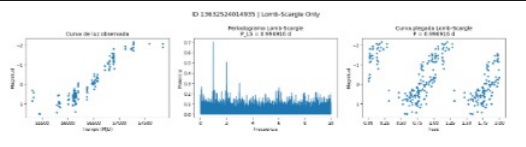
\includegraphics[width=1\linewidth]{../VVVResults/LS_Star_41.png}
    \caption{Esta estrella, a lo largo de 2000 días, sólo aumentó en magnitud. LS le encuentra un periodo de un día, 
    y pretende que su magnitud oscila. }
    \label{STAR41VVV}
\end{figure}

\begin{figure}[h]
    \centering
    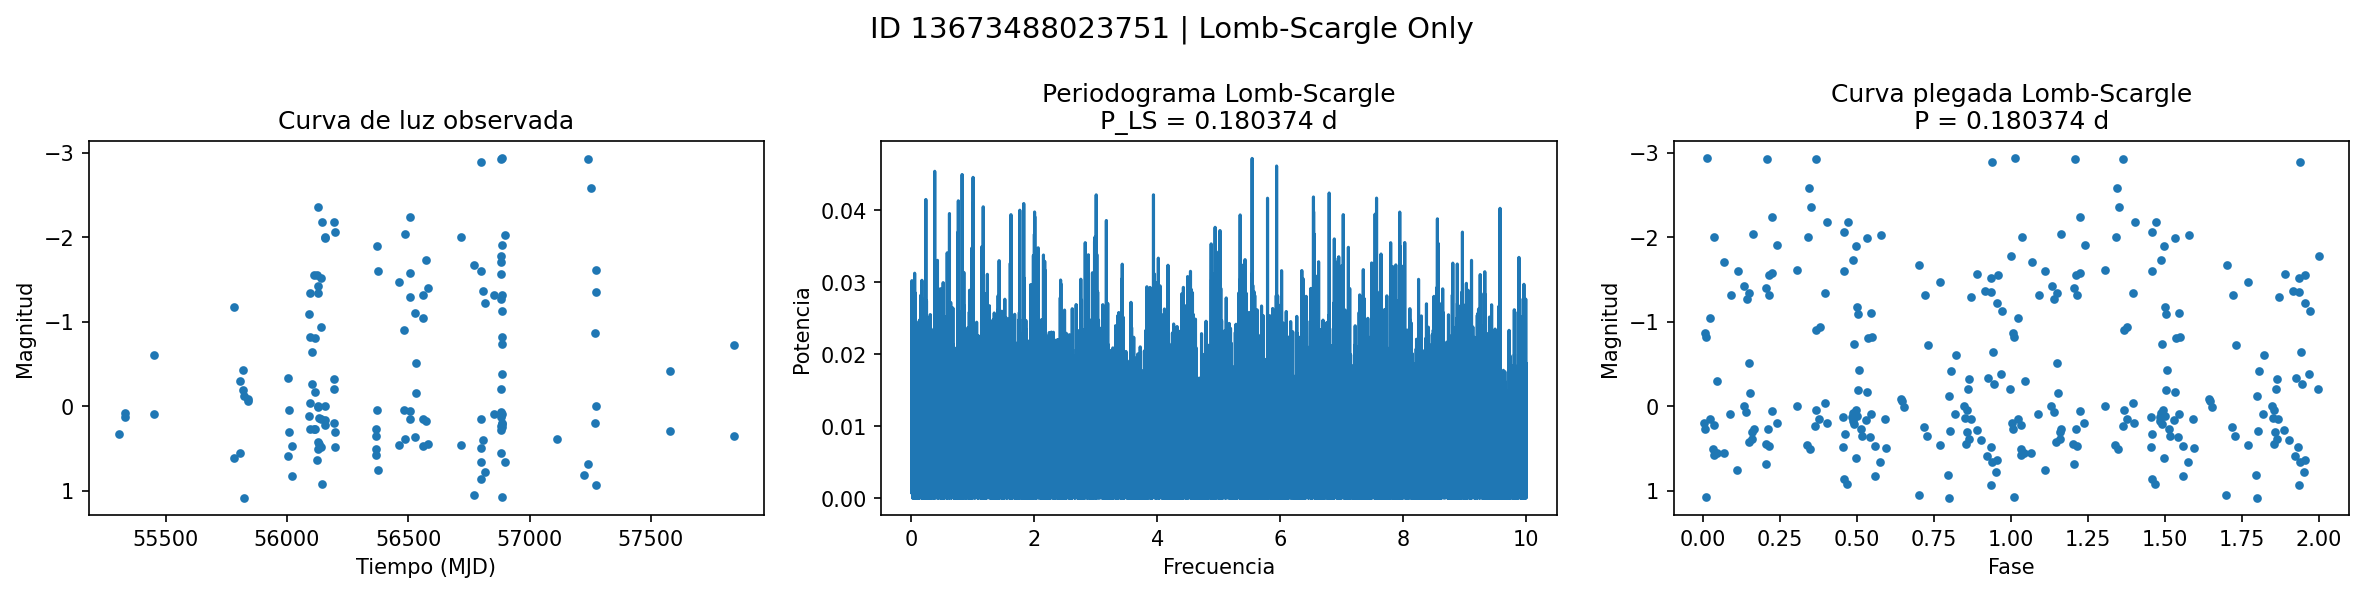
\includegraphics[width=1\linewidth]{../VVVResults/LS_Star_12.png}
    \caption{Estrella con una búsqueda de frecuencias llena de ruido, en la que no se puede discernir mucho. 
    Su curva de luz plegada no dice nada sobre la estrella, y su curva de luz observada parece falta de datos.}
    \label{STAR12VVV}
\end{figure}

\begin{figure}[h]
    \centering
    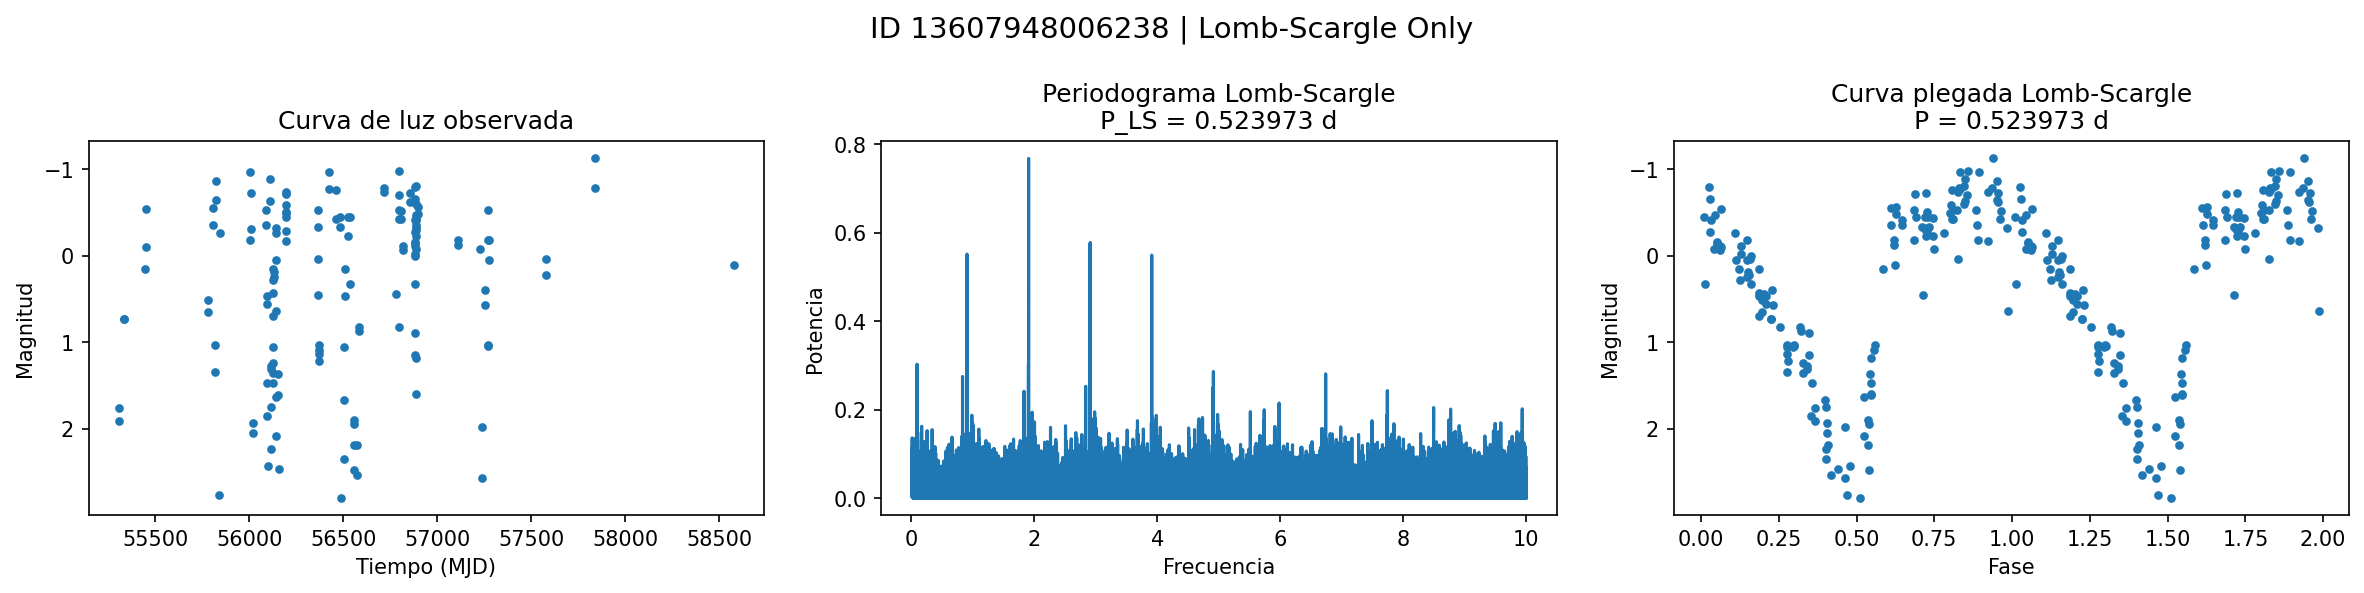
\includegraphics[width=1\linewidth]{../VVVResults/LS_Star_14.png}
    \caption{Estrella con muy pocos datos de inicio. La búsqueda de LS es prácticamente solo ruido, ya que 
    tiene picos de potencia similares en distintas partes del espectro de frecuencias. Su curva plegada parece coherente, 
    pero viendo los resultados de LS, otro periodo hubiera hecho algo muy similar.}
    \label{STAR14VVV}
\end{figure}

En general, las primeras 20 estrellas de VVV son estrellas complicadas de resolver, mientras que OGLE tiene un cuerpo de estrellas
mucho más limpias. El autor no conoce mucho la diferencia, pero una búsqueda rápida en internet muestra que, mientras que OGLE
trabaja en el óptico, VVV trabaja en el infrarrojo, y que VVV mapea el bulbo de la vía láctea en conjunto mientras que OGLE 
puede observar la misma región del cielo por años y años. No es sorprendente que sus datos aparezcan más finos, entonces. 

Por otro lado, podemos corroborar lo que se ha dicho en informes anteriores: al tratar con métodos computacionales, siempre
se obtendrán resultados aunque no exista nada real de por medio. Las primeras 20 estrellas de VVV confirman que, aún con
sets de datos débiles, el computador va a dar un resultado. Es posible que, tras volver a correr el código, se encuentre
otro periodo para la misma estrella, puesto que pocos datos y una periodicidad poco clara llevan a que el computador no 
pueda separar una frecuencia satisfactoriamente y con seguridad: el ruido es dominante, especialmente al compararlo con 
estrellas mucho más limpias. 

Esta primera parte del análisis nos deja ver que Lomb Scargle es un buen método para distinguir una estrella variable de una 
no variable, ya que es capaz de separar muy bien una frecuencia y una curva de luz coherente con los datos que se le proporcionan.
Si los datos no tienen nada, lo que muestre LS no tendrá nada tampoco, cosa que también aplica para la cantidad de datos. Si 
tenemos pocos datos, LS encontrará el resultado más coherente para lo que le demos, pero será evidente que los datos son 
insufucientes por el ruido que muestra el método y por las curvas de luz que encuentra. Es decir, la astrofísica observacional
toma años en dar resultados, puesto que no se puede ser mucho más efectivo que esto para encontrar resultados con un tamaño de 
datos determinado. Solo se puede ser más refinado con el método. 

\subsection{Mínima Entropía}

Con la manera de visualizar resultados de Lomb Scargle ya vista, podemos hablar de mínima entropía. Este método no es un 
método que se encuentre en alguna librería; es de implementación personal. Es mucho más demandante computacionalmente, 
y es más complejo en general. 

En términos generales, es una gran confirmación para Lomb-Scargle, ya que, al menos en los resultados encontrados, 
llega a replicar perfectamente los resultados de este. Por esto mismo nos vamos a centrar en los resultados un poco más extraños 
que llegamos a encontrar: las estrellas 4, 8, 10, 14 y 17, así como un caso curioso que se repite en las estrellas 
3, 4, 6, 7, 11, 12, 13, 15, 16, 18, 19 y 20.

Nótense dos cosas: La estrella 4 está repetida, y en iteraciones anteriores(que tenían una visualización incómoda de M.E)
se encontraron curvas plegadas ordenadas por bloques y no como un continuo

\section{Conclusiones}


\section*{Comentarios al margen}


\end{document}